\chapter{What is algebra?}

Algebra is the study of equations, for the most part equations involving variables.
That is because applications have unknowns and if 
the shape of the equation can tell us anything about the 
options to solve it, we shall want to take advantage of this.
Witness how we solve $ax^2+bx+c=0$ in one strategy despite it covering 
an infinite number of equations. Basic though it may seem that solution illustrates
the general arc of an algebra investigation.
\begin{enumerate}
    \item What numbers lead to solutions existing? Do we need to invent $\sqrt{2}$
    $i$, and possibly others?
    \item If solutions exists, what algorithms find them? Complete the square, 
        use a stock quadratic formula? Gaussian eliminate?
    \item When multiple solutions, relate them to one another to simplify the answer.  
    E.g.\ $\pm \sqrt{2}$, shift answers to a null space, use a basis.  Go 
    back to 1 with these relations.
\end{enumerate}
Childhood is mostly problem 1.  Children learn to count, find distances of
length $\sqrt{2}$, learn about imaginary numbers and $\pi$.  The shift to $\pi$
signals the shift to question 2 because $\pi$ is such an approximate fiddly
number that it makes sense to leave it alone moving it round solely by rules of
algebra until the end when we might replace with with 3.14; it is treated like a
variable. High school algebra is nearly all question 2, and mostly following al
Khwarizmi's \emph{al Jabr}---the method of balancing parts, which today is called 
Algebra.  Move over Euclid, al Khwarizmi's method made
people money, settled land disputes, calculated grain totals and arguably 
did more to make math a necessity for average people than any other source.
His name has passed down to modern life as the word \emph{algorithm}.
Then students are told of 
that polynomials of degree $d$ have $d$ complex
roots.  Perhaps because some non-algebraist call this fact ``the fundamental theorem
of algebra'' (it's not) this seems to be the end of algebra for most students having 
never reach a type 3 algebra problem, and with that no iterated use of 1, and 2 techniques.

If you do get to a type 3 problem the next example will be groups---the
relations between the roots of polynomials.  This is where the heavy weights get
involved: Lagrange makes a formula for quartic polynomials from a primitive
concept of groups using type 3 reasoning.  Gauss shows that construction by
ruler and compass requires only square-roots explaining that their type 3 algebra 
will be nilpotent (by today's langauge). Abel finds that $x^5-x+1=0$ has no 
solution by radicals by exposing contradictions that type 3 numbers 
would force on calculus.  Galois characterizes all polynomials that can be solved 
by radicals by describing what their type 3 algebra would look like.

Here I should settle a confusion in the subject.  Abel and Galois did 
not show that the quintic has no solutions!  That would fly in the 
face of  Gauss' ``fundamental theorem 
of algebra'' (a 5th degree polynomial has 5 complex roots).  
What Abel and Galois proved is that roots of these polynomials 
are not always linear combinations of radicals, $\sqrt{2}$, $\sqrt[3]{7}$ and 
etc.  This is just the latest in a long line of type 1 algebra problems.  First 
$x+5=2$ provoked a need for negatives, $5x=2$ required fractions, $x^2=2$ 
needs irrational numbers, and $x^5-x+1=0$ needs some numbers beyond 
those that can be written like this
\[
    \sum_i \frac{a_i}{b_i}\sqrt[n_i]{\alpha_i}.
\]
Had this been true we would also know an algorithm, some inductive process, 
to reduce all factoring to the form $x^n=\alpha$.  So this no-go theorem 
says you need more subtle numbers and more subtle algorithms. Back to the 
drawing board with type 1 and 2 problems.

If you wonder, doesn't the fundamental theorem of algebra already 
give us those numbers, i.e.\ complex numbers?  Sure, but algebra has never 
deeply cared about the data structure to write down the roots.  In fact we 
pride ourselves on finding $x=\sqrt{2}$ rather than $x\approx 1.42$.
Maybe personal pride shouldn't be a motive.  But ask your computer to 
use approximation methods 
compute the eigenvalues of 
\begin{align*}
    \begin{bmatrix}
        1 & -1 \\
        1 & -1
    \end{bmatrix}
\end{align*}
Even with 64 bit floating point precision in Julia, my computer printed out 
\begin{lstlisting}
julia> eigvals([1 -1; 1 -1])
2-element Vector{ComplexF64}:
2.2371143170757382e-17 - 1.570092458683775e-16im
2.2371143170757382e-17 + 1.570092458683775e-16im      
\end{lstlisting}
In reality our matrix has but only one eigenvalue $0$, but this computation would 
even allow us to invert this non-invertible matrix.  This gets at the heart of 
serious problem with approximations.  Algebraic solutions often change in an instant
with the nearby approximate solutions begin quite different.  Think 
merely of $x^2=0$.  This is near to both $x^2+0.0001$ and $x^2-0.0001$.  Both give 
a pair of distinct roots only at $x^2+0=0$ do we get the correct answer.
Algebraic solutions are as necessary today as ever before.





Algebra today is taught chronologically by example. 
First groups, then rings, then fields, then modules,
then bigger groups, then crazier rings, then fusing groups and rings with
outside influences like topology, analysis, and geometry.  So today there are
few general-practice algebraist.  There are instead geometric group theorist,
algebraic geometers, commutative ring theorist, non-associative algebraist,
computational algebraist, and even those topics are too general for any one
theorist to master.  

It bucks tradition and a century of pedagogy to change this 
but if there is to be a generalist algebraist, or if we are to make 
algebra accessible to non-specialist, it seems necessary to explore algebra 
as a unified topic with many branches that exploit some details.
This text explores algebra with aim.

\section{Everything is variable}
You probably already know every color, shape, and pattern of 
equation you will ever need.  Compare these two equations
\begin{align*}
    x^2+y^2 & \equiv 0 \pmod{541} 
    & 
    \frac{\partial^2 f}{\partial x^2}+\frac{\partial^2 f}{\partial y^2} & =0.
\end{align*}
Can you stop yourself from seeing them as related?
These equations concern entirely different things.  On the left $0$ can 
equal 541.  On the right $0$ is functions on the $xy$-plane.
Yet, the similarities as equations shine through.  Why? Is it because $0$, 
$+$, and  powers of $2$ are general concepts, ``abstractions''.  This doesn't connect them to
polarizing art movements nor render the concept inapplicable.  Abstract here,
and everywhere, means to study by limited attributes.  That's how we do all
math and science.  So when we abstract the equation on the left we forget
about mod 541 and the precise meaning of these numbers.  On the right we forget
about functions and the notions of derivatives.  We are left with just $0$, 
$+$, and squares and where they sit.  We abstract both to a common equation
\[
    x^2+y^2=0.
\]
In fact, even the equality was an abstraction which could vary from context to context.
With such flexibility a small number of symbols and their grammar are enough to capture 
the huge variety of equations we encounter in real life.

\begin{quote}
    \textbf{The power of algebra is that every symbol 
    in an equation is a variable, especially the equals sign.}
\end{quote}

\section{Inventing numbers}
Now since every symbol in an equation is a variable we have new powers 
to solve equations.  Look to the humble 
\[
    x^2+1=0.
\]
By our own view, right now this is nothing but variables, so it means nothing to
solve this.  But, drop this into a context such as decimal numbers $\mathbb{R}$
and the understanding is to replace $1\defeq 1.0$, $0\defeq 0.0$, $+$ is
substituted for addition of decimals, and square is by multiplying decimals.
Equality now means two equal decimals, or in practice two decimal numbers that are close enough 
to be considered equal.  The only remaining unknown is $x$, but as everyone 
knows, $0\leq x$ or $x<0$ so in both cases $-1<0\leq x^2$.

The power of variable everything is that we are not stuck with the real numbers.
Let us replace everything with complex numbers $\mathbb{C}$. Substitute $0\defeq
0+0i$, $1=1+0i$, $(a+bi)+(c+di)\defeq (a+b)+(c+d)i$, and
$(a+bi)^2=(a^2-b^2)+2abi$.  Now we find $\pm i$ are the solutions. Solutions do
exist!  Since they exist we can return to a problem and ask if the solutions we 
found will do the job.  Maybe not, or maybe we should revisit our models and 
see these solutions as predicting the presence of previously unknown realities.

Why stop here? Quaternions have $\hat{\i}^2=\hat{\j}^2=\hat{k}^2=-1$;
so, at least 6 solutions to $x^2+1=0$.  Even more.  Try $(2\times 2)$-matrices, I
bet you can find infinitely many matrices $M$ where $M^2=-I_2$.  This is the method
of algebra: dream up new numbers that might be used to solve equations.  Alter
their properties, e.g.\ drop the order of real numbers and you can get complex
solutions.  Drop commutative multiplication of complex numbers and you might get
infinite solutions.  Learn enough by this process and we can begin to predict if
solutions are to be expected and fathom algorithms to find them when they do
exist. When the solutions become infinite we find ways to parameterize them with
smaller data such as a basis.

Don't forget equality is variable too!  Suppose we wanted to solve $x^{541}+x+1=0$
using only integers.  Replace equality 
with $\equiv$ modulo 2 and ask for a whole number $x$ that solves
\begin{align*}
    x^{541}+x+1\equiv 0\pmod{2}.
\end{align*}
All integers in this equality become either $0$ or $1$, but neither will solve 
this equation.  By varying equality we confirm there are no solutions.

This is why so much of algebra today is concerned with making new numbers and 
searching out which equalities (congruences) can be used on new numbers.  It is 
the front line of algebra, the first question that must be concurred.  And it part 
of why so much research on algebra doesn't even feature solving equations because 
the goal is to have numbers ready for whatever equations show up.

\begin{quote}
    \textbf{The first method of algebra is to invent numbers: their constants, their 
    operations, their rules.  We call these ``algebras''.}
\end{quote}

\section{Computation}
Algebra is the computational wing of mathematics.  

Look to calculus.
We obviously work with limits and derivatives to recover Rolle's theorem 
and the significance of $f'(x)=0$.  But when we want to find such $x$ we
inevitably are left to solve equations, like $x^2-x-3=0$, which we do by algebra.  

Switch to topology.   Roll up a stretchy sheet of plastic along the following 
Van Kampen patterns  viewed in Figure~\ref{fig:vanKampen} to make a torus $\mathbb{T}^2$ 
and a Klein bottle $\mathbb{K}$.  These are different, right?  Why?  Of course we use topology 
to prove the interesting bit, like the Seifert-van Kampen theorem: the loops 
$\pi_1(M^2)$ on a surfaces $M^2$ can each be described as a sequence of blue loops $b$ and red loops $r$.
Loops that contract to nothing can be read along the boundary.  Hence,
\begin{align*}
    \pi_1(\mathbb{T}^2) &= \text{ words over }\{b,r\} \text{ rewritten by }br=rb;
    \\
    \pi_1(\mathbb{K}^2) &= \text{ words over }\{b,r\} \text{ rewritten by } r=brb. 
\end{align*}
We use algebra to compute that those numbers are not the same so neither are the two spaces.
\begin{figure}[!htbp]
    \centering
\begin{tikzpicture}
    \node (T) at (-3,0) {\begin{tikzpicture}
        \fill[color=black!25] (0,0) rectangle (2,2);
        \draw[thick,->, red] (0,0) -- ++(2,0);
        \draw[thick,->,red] (0,2) -- ++(2,0);
        \draw[thick,->>, blue] (0,0) -- ++(0,2);
        \draw[thick,->>,blue] (2,0) -- ++(0,2);
    \end{tikzpicture}};
    \node (K) at (3,0) {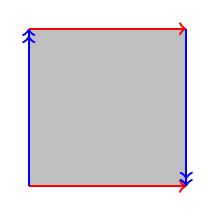
\begin{tikzpicture}
        \fill[color=black!25] (0,0) rectangle (2,2);
        \draw[thick,->, red] (0,0) -- ++(2,0);
        \draw[thick,->,red] (0,2) -- ++(2,0);
        \draw[thick,->>, blue] (0,0) -- ++(0,2);
        \draw[thick,->>,blue] (2,2) -- ++(0,-2);
    \end{tikzpicture}};

    \node (Tv) at (-3,-3) {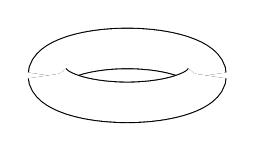
\begin{tikzpicture}[yscale=cos(70)]
        \draw[double distance=5mm] (0:1) arc (0:180:1);
        \draw[double distance=5mm] (180:1) arc (180:360:1);
      \end{tikzpicture}};
    \node (Kv) at (3,-3) {\begin{tikzpicture}[scale=0.25,use Hobby shortcut]
        \draw ([closed,blank=soft]0,0)
        \foreach \pt in {
        (-2,2),
        (2,2),
        (2,-2),
        (-2,-2),
        ([blank]-2,-1),
        (-1,-1),
        (1,-2),
        ([blank=soft]1,2),
        ([blank=soft]-1,1),
        (-3,3),
        (6,4.5),
        (4.5,-4.5),
        (-2.5,-6)
        } {
        .. ++\pt
        };
        % \draw[dashed,use previous hobby path={invert soft blanks}];
        \draw (0,0) .. +(-1,-1) .. ++(-2,-1);
        \draw[dashed] (0,0) .. +(-1,-.75) .. ++(-2,-1);
        \draw (-2.45,-3.9) .. +(3.3,-.75) .. (4.2,-3.95);
        \draw[dashed] (-2.45,-3.9) .. +(4.3,.5) .. (4.2,-3.95);
        \end{tikzpicture}};

        \draw[thick,->] (T) -- (Tv);
        \draw[thick,->] (K) -- (Kv);
    \end{tikzpicture}
    \caption{A torus and Klein bottle, with thanks to 
    \url{https://tex.stackexchange.com/q/77606/86}.}\label{fig:vanKampen}
\end{figure}

Other fields?  How many times in applied math, number theory, or combinatorics
do we end up solving something even if just a linear equation, in order to get 
a final answer?  You don't have to be convinced but the evidence is there.

Yet most of us do not want to be computers.  So what does an algebraist do 
when the questions come down to computing?  We put our energy into crafting 
algorithms to solve these problems.  In fact the word ``algorithm'' comes 
from al Khwarizmi whose influential book \emph{al Jabr} (the method of parts)
gave use the first detailed explanations of algebra.  Half of that book 
is a list of story problems solved by various algorithms in algebra.
If you are concerned that this now trends to computer science, well know that 
computer science cares more about the data structures than about any algorithms.
Just like counting get faster with an abacus, algebraic algorithms get better 
with data structures.  So these two worlds interact but care deeply about 
different parts of the problem.